\documentclass{standalone}
\usepackage{tikz}
\usetikzlibrary{patterns, positioning}
\usepackage[sfdefault]{ClearSans} %% option 'sfdefault' activates Clear Sans as the default text font
\usepackage[T1]{fontenc}

\begin{document}
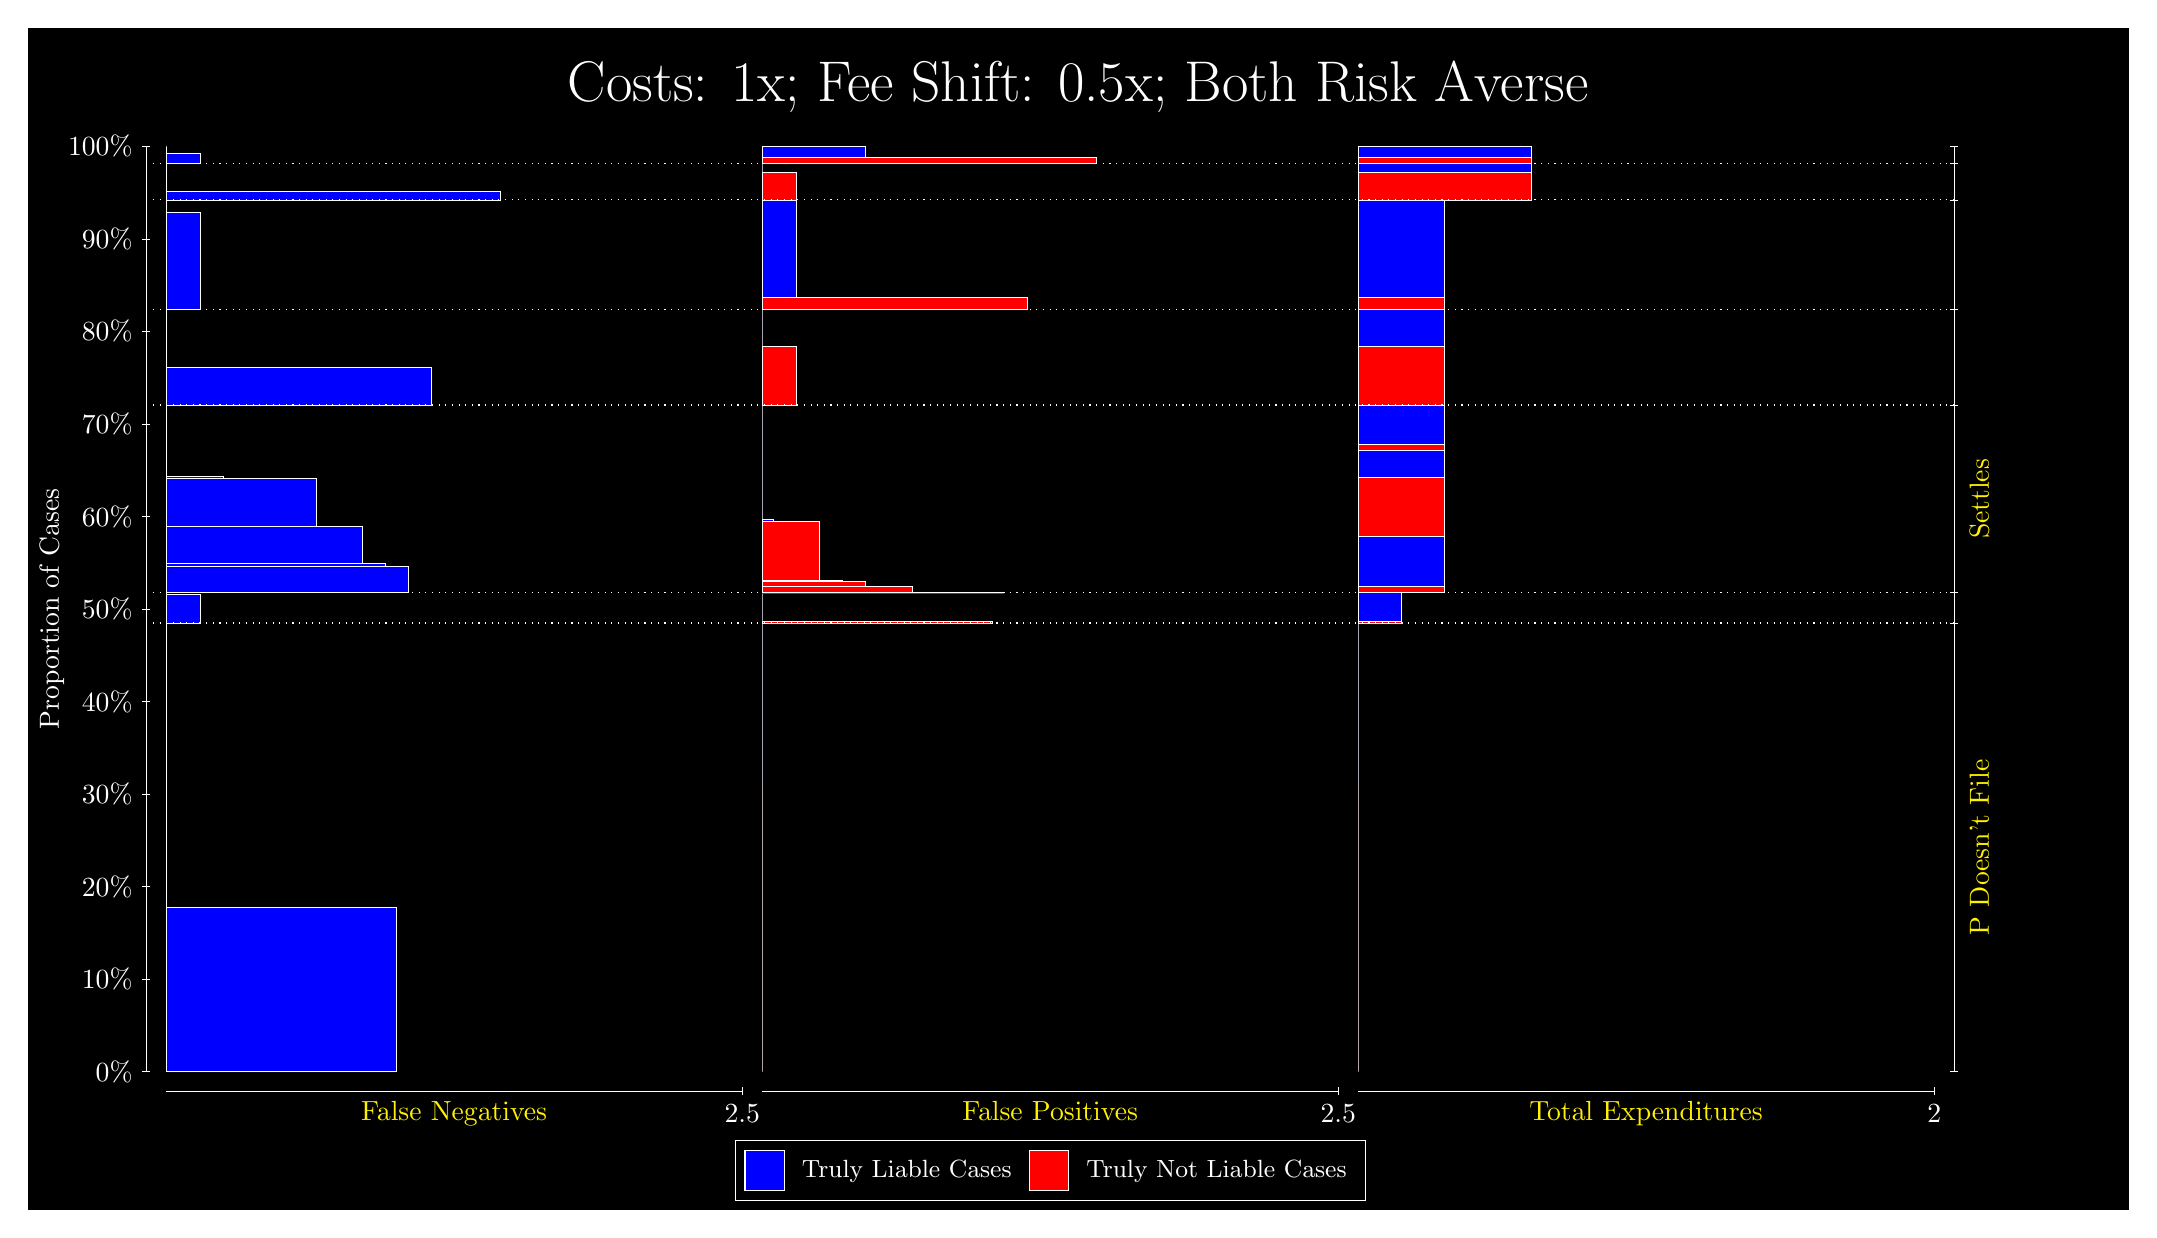
\begin{tikzpicture}
\draw[fill=black] (0,0) rectangle (26.667,15);
\draw[text=white] (0,13.5) rectangle (26.667,15) node[midway] {\huge Costs: 1x; Fee Shift: 0.5x; Both Risk Averse};
\draw[white, very thin] (1.5,1.75) -- (1.5,13.5);
\node[rotate=90, text=white, anchor=center] at (0.3, 7.625) {Proportion of Cases};
\draw[white, very thin] (1.45,1.75) -- (1.55,1.75);
\node[text=white, anchor=east] at (1.45, 1.75) {0\%};
\draw[white, very thin] (1.45,2.925) -- (1.55,2.925);
\node[text=white, anchor=east] at (1.45, 2.925) {10\%};
\draw[white, very thin] (1.45,4.1) -- (1.55,4.1);
\node[text=white, anchor=east] at (1.45, 4.1) {20\%};
\draw[white, very thin] (1.45,5.275) -- (1.55,5.275);
\node[text=white, anchor=east] at (1.45, 5.275) {30\%};
\draw[white, very thin] (1.45,6.45) -- (1.55,6.45);
\node[text=white, anchor=east] at (1.45, 6.45) {40\%};
\draw[white, very thin] (1.45,7.625) -- (1.55,7.625);
\node[text=white, anchor=east] at (1.45, 7.625) {50\%};
\draw[white, very thin] (1.45,8.8) -- (1.55,8.8);
\node[text=white, anchor=east] at (1.45, 8.8) {60\%};
\draw[white, very thin] (1.45,9.975) -- (1.55,9.975);
\node[text=white, anchor=east] at (1.45, 9.975) {70\%};
\draw[white, very thin] (1.45,11.15) -- (1.55,11.15);
\node[text=white, anchor=east] at (1.45, 11.15) {80\%};
\draw[white, very thin] (1.45,12.325) -- (1.55,12.325);
\node[text=white, anchor=east] at (1.45, 12.325) {90\%};
\draw[white, very thin] (1.45,13.5) -- (1.55,13.5);
\node[text=white, anchor=east] at (1.45, 13.5) {100\%};

\draw[white, very thin] (24.457,1.75) -- (24.457,13.5);
\draw[white, very thin] (24.407,1.75) -- (24.507,1.75);
\node[anchor=west] at (24.407, 1.75) {};
\draw[white, very thin] (24.407,7.4459) -- (24.507,7.4459);
\node[anchor=west] at (24.407, 7.4459) {};
\draw[white, very thin] (24.407,7.8314) -- (24.507,7.8314);
\node[anchor=west] at (24.407, 7.8314) {};
\draw[white, very thin] (24.407,10.215) -- (24.507,10.215);
\node[anchor=west] at (24.407, 10.215) {};
\draw[white, very thin] (24.407,11.431) -- (24.507,11.431);
\node[anchor=west] at (24.407, 11.431) {};
\draw[white, very thin] (24.407,12.82) -- (24.507,12.82);
\node[anchor=west] at (24.407, 12.82) {};
\draw[white, very thin] (24.407,13.281) -- (24.507,13.281);
\node[anchor=west] at (24.407, 13.281) {};
\draw[white, very thin] (24.407,13.5) -- (24.507,13.5);
\node[anchor=west] at (24.407, 13.5) {};

\draw[white, very thin, fill=blue] (1.75,1.75) rectangle (4.6775,3.8304);
\draw[white, very thin, fill=red] (1.75,3.8304) rectangle (1.75,7.4459);
\draw[white, very thin, fill=blue] (1.75,7.4459) rectangle (2.1891,7.81);
\draw[white, very thin, fill=red] (1.75,7.81) rectangle (1.75,7.8314);
\draw[white, very thin, fill=blue] (1.75,7.8314) rectangle (4.8239,8.1661);
\draw[white, very thin, fill=blue] (1.75,8.1661) rectangle (4.5312,8.1991);
\draw[white, very thin, fill=blue] (1.75,8.1991) rectangle (4.2384,8.6711);
\draw[white, very thin, fill=blue] (1.75,8.6711) rectangle (3.6529,9.2826);
\draw[white, very thin, fill=blue] (1.75,9.2826) rectangle (3.3602,9.2832);
\draw[white, very thin, fill=blue] (1.75,9.2832) rectangle (2.4819,9.3085);
\draw[white, very thin, fill=red] (1.75,9.3085) rectangle (1.75,10.215);
\draw[white, very thin, fill=blue] (1.75,10.215) rectangle (5.1167,10.69);
\draw[white, very thin, fill=red] (1.75,10.69) rectangle (1.75,11.431);
\draw[white, very thin, fill=blue] (1.75,11.431) rectangle (2.1891,12.668);
\draw[white, very thin, fill=red] (1.75,12.668) rectangle (1.75,12.82);
\draw[white, very thin, fill=blue] (1.75,12.82) rectangle (5.9949,12.925);
\draw[white, very thin, fill=red] (1.75,12.925) rectangle (1.75,13.281);
\draw[white, very thin, fill=blue] (1.75,13.281) rectangle (2.1891,13.417);
\draw[white, very thin, fill=red] (1.75,13.417) rectangle (1.75,13.5);
\draw[white, very thin, fill=red] (9.3189,1.75) rectangle (9.3189,5.3656);
\draw[white, very thin, fill=blue] (9.3189,5.3656) rectangle (9.3189,7.4459);
\draw[white, very thin, fill=red] (9.3189,7.4459) rectangle (12.246,7.4673);
\draw[white, very thin, fill=blue] (9.3189,7.4673) rectangle (9.3189,7.8314);
\draw[white, very thin, fill=red] (9.3189,7.8314) rectangle (12.393,7.8328);
\draw[white, very thin, fill=red] (9.3189,7.8328) rectangle (11.515,7.8329);
\draw[white, very thin, fill=red] (9.3189,7.8329) rectangle (11.222,7.9093);
\draw[white, very thin, fill=red] (9.3189,7.9093) rectangle (10.636,7.9785);
\draw[white, very thin, fill=red] (9.3189,7.9785) rectangle (10.344,7.9826);
\draw[white, very thin, fill=red] (9.3189,7.9826) rectangle (10.051,8.7379);
\draw[white, very thin, fill=blue] (9.3189,8.7379) rectangle (9.4652,8.7633);
\draw[white, very thin, fill=blue] (9.3189,8.7633) rectangle (9.3189,10.215);
\draw[white, very thin, fill=red] (9.3189,10.215) rectangle (9.758,10.956);
\draw[white, very thin, fill=blue] (9.3189,10.956) rectangle (9.3189,11.431);
\draw[white, very thin, fill=red] (9.3189,11.431) rectangle (12.686,11.583);
\draw[white, very thin, fill=blue] (9.3189,11.583) rectangle (9.758,12.82);
\draw[white, very thin, fill=red] (9.3189,12.82) rectangle (9.758,13.176);
\draw[white, very thin, fill=blue] (9.3189,13.176) rectangle (9.3189,13.281);
\draw[white, very thin, fill=red] (9.3189,13.281) rectangle (13.564,13.364);
\draw[white, very thin, fill=blue] (9.3189,13.364) rectangle (10.636,13.5);
\draw[white, very thin, fill=red] (16.888,1.75) rectangle (16.888,5.3656);
\draw[white, very thin, fill=blue] (16.888,5.3656) rectangle (16.888,7.4459);
\draw[white, very thin, fill=red] (16.888,7.4459) rectangle (17.437,7.4673);
\draw[white, very thin, fill=blue] (16.888,7.4673) rectangle (17.437,7.8314);
\draw[white, very thin, fill=red] (16.888,7.8314) rectangle (17.986,7.9093);
\draw[white, very thin, fill=blue] (16.888,7.9093) rectangle (17.986,8.5468);
\draw[white, very thin, fill=red] (16.888,8.5468) rectangle (17.986,9.3021);
\draw[white, very thin, fill=blue] (16.888,9.3021) rectangle (17.986,9.6369);
\draw[white, very thin, fill=red] (16.888,9.6369) rectangle (17.986,9.7101);
\draw[white, very thin, fill=blue] (16.888,9.7101) rectangle (17.986,10.215);
\draw[white, very thin, fill=red] (16.888,10.215) rectangle (17.986,10.956);
\draw[white, very thin, fill=blue] (16.888,10.956) rectangle (17.986,11.431);
\draw[white, very thin, fill=red] (16.888,11.431) rectangle (17.986,11.583);
\draw[white, very thin, fill=blue] (16.888,11.583) rectangle (17.986,12.82);
\draw[white, very thin, fill=red] (16.888,12.82) rectangle (19.083,13.176);
\draw[white, very thin, fill=blue] (16.888,13.176) rectangle (19.083,13.281);
\draw[white, very thin, fill=red] (16.888,13.281) rectangle (19.083,13.364);
\draw[white, very thin, fill=blue] (16.888,13.364) rectangle (19.083,13.5);
\draw[white, dotted] (1.5,7.4459) -- (24.457,7.4459);
\draw[white, dotted] (1.5,7.8314) -- (24.457,7.8314);
\draw[white, dotted] (1.5,10.215) -- (24.457,10.215);
\draw[white, dotted] (1.5,11.431) -- (24.457,11.431);
\draw[white, dotted] (1.5,12.82) -- (24.457,12.82);
\draw[white, dotted] (1.5,13.281) -- (24.457,13.281);
\draw[white, very thin] (1.75,1.5) -- (9.0689,1.5);
\node[text=yellow, anchor=north] at (5.4094, 1.5) {False Negatives};
\draw[white, very thin] (9.0689,1.45) -- (9.0689,1.55);
\node[text=white, anchor=north] at (9.0689, 1.45) {2.5};

\draw[white, very thin] (9.3189,1.5) -- (16.638,1.5);
\node[text=yellow, anchor=north] at (12.978, 1.5) {False Positives};
\draw[white, very thin] (16.638,1.45) -- (16.638,1.55);
\node[text=white, anchor=north] at (16.638, 1.45) {2.5};

\draw[white, very thin] (16.888,1.5) -- (24.207,1.5);
\node[text=yellow, anchor=north] at (20.547, 1.5) {Total Expenditures};
\draw[white, very thin] (24.207,1.45) -- (24.207,1.55);
\node[text=white, anchor=north] at (24.207, 1.45) {2};

\node[text=yellow, centered, rotate=90] at (24.777, 4.598) {P Doesn't File};

\node[text=yellow, centered, rotate=90] at (24.777, 9.0232) {Settles};





\draw (12.978300999999998,1.5) node[draw=none] (baseCoordinate) {};
\begin{scope}[align=center]
        \matrix[scale=0.5, draw=white, below=0.5cm of baseCoordinate, nodes={draw}, column sep=0.1cm]{
            \node[rectangle, draw, minimum width=0.5cm, minimum height=0.5cm, fill=blue] {}; &
            \node[draw=none, font=\small, text=white] (B) {Truly Liable Cases}; &
            \node[rectangle, draw, minimum width=0.5cm, minimum height=0.5cm, fill=red] {}; &
            \node[draw=none, font=\small, text=white] (B) {Truly Not Liable Cases}; \\
            };
\end{scope}

\end{tikzpicture}
\end{document}